% Chapter 2

\chapter{Traducción de problemas NP}
\label{Chapter2}
\lhead{Capítulo 2. \emph{Traducción de problemas NP}}
Este capítulo describe el diseño de una herramienta capaz de transformar una
descripción de un problema en lógica de segundo orden 
en un problema de planificación de clase de complejidad equivalente. 
Primero se presenta una perspectiva a alto nivel de lo que de

\section{Perspectiva general}
\begin{figure}[h!]
\centering
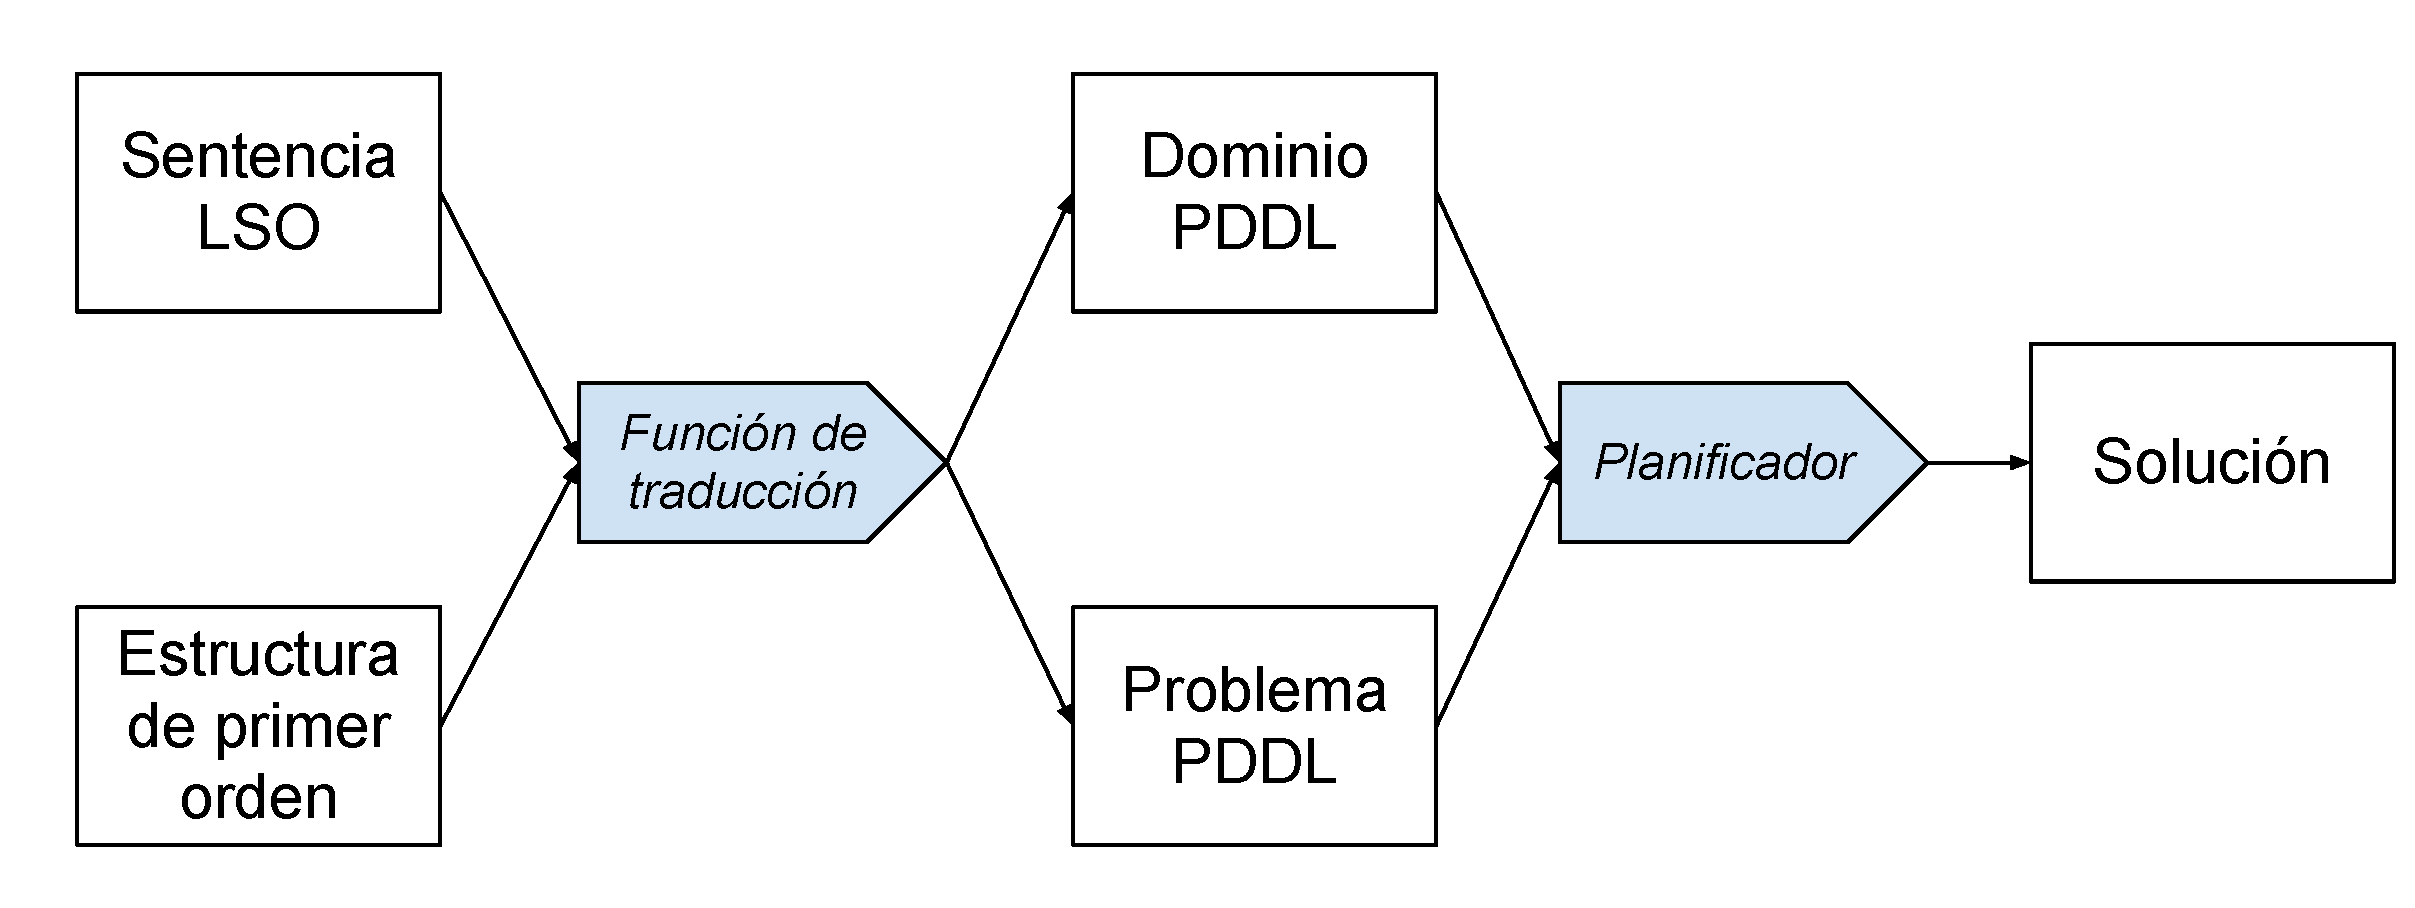
\includegraphics[width=\textwidth]{figuras/esquema_herramienta.pdf}
\caption{Posible estado para un problema en \textit{mundo de bloques}.}
\label{esquema_herramienta}
\end{figure}

\section{Diseño del lenguaje}


\section{Reducción base}
\subsection{Reducción del dominio}
\subsection{Reducción del problema}

\section{Propiedades formales}
\subsection{Demostración: reducción a STRIPS}

\begin{theorem}
The function $f_{\sigma,\Phi}$ is a polytime reduction from $\mod[\Phi]$
into STRIPS-1.
\end{theorem}

\begin{proof}
	The statement to show is that
$\A\models(\exists R_1^{a_1})\cdots(\exists R_k^{a_k})\psi$ iff
there is a plan that achieves the fluent $\FT[\psi]$.The proof is by structural induction on the FOL-sentence $\psi$ starting from the simplest sentences and building 
towards the more complex ones. \\

Para toda subformula $\theta$ de $\psi$, y toda interpretacion $(\A,i)$ de $\A$:\\ \\
$ $ \hspace*{3cm} $(\A,i) \models \theta(\overline{X}) \iff$ a plan exists for $\FT[\theta](\overline{X})$ \\

Proof by mutual implication.
We start proving:\\ \\
$ $ \hspace*{3cm} $(\A,i) \models \theta(\overline{X}) \Rightarrow $ a plan exists for $\FT[\theta](\overline{X})$ \\
\begin{itemize}
		\item Caso base: $\theta$ is a literal. $\theta = P(X)$ 
		
		Prueba por casos:
			\begin{itemize}
				\item Caso 0: $P(\overline{X})$ $\epsilon$ $\sigma$
				
				\begin{tabular}{@{}p{1mm}p{1mm}p{11cm}}	
						& & $\A \models P(\overline{X})$\\
						$\eq$ & & $<(A,i)$ es una interpretacion de $\A>$ \\
						& & $(A,i) \models P(\overline{X})$ \\
						$\eq$ & & $<$Definicion de interpretacion$>$\\
						& & $i(\overline{X})$ $\epsilon$ $P^{\A}$\\
						$\Rightarrow$ & & $<$ La situacion inicial (Init) consiste de fluents describiendo el valor de 
									  verdad de todas las relaciones en $\A$$>$\\
						& & $P(\overline{X})$ $\epsilon$ $Init$ \\
						$\eq$ & & $<$ Hy un plan de cero pasos para $\theta(\overline{x})>$\\
						& & $\FT[\theta](\overline{X})$ tiene solucion
					\end{tabular}
					
					
				\item Caso 1: $P(\overline{X})$ $\epsilon$ $\Phi$
				
					  Falta
			\end{itemize}
			
		\item Caso inductivo:
			\begin{itemize}
				\item Caso 0: $\theta = \neg P(\overline{X})$ (Como esta definido en el paper la negacion esta solo en los literales)
				
				\begin{tabular}{@{}p{1mm}p{1mm}p{11cm}}	
						& & $\A \models \neg P(\overline{X})$\\
						$\eq$ & & $<(A,i)$ es una interpretacion de $\A>$ \\
						& & $(A,i) \models \neg P(\overline{X})$ \\
						$\eq$ & & $<$Definicion de interpretacion$>$\\
						& & $i(\overline{X})$ $\epsilon$ ${\neg P}^{\A}$\\
						$\Rightarrow$ & & $<$ La situacion inicial (Init) consiste de fluents describiendo el valor de 
									  verdad de todas las relaciones en $\A$ (La negacion de un literal es tomado como
									  un fluent nuevo)$>$\\
						& & $P(\overline{X})$ $\epsilon$ $Init$ \\ 
						$\eq$ & & $<$ Hy un plan de cero pasos para $\theta(\overline{x})>$\\
						& & $\FT[\theta](\overline{X})$ tiene solucion
				\end{tabular}
					
				\item Caso 1: $\theta = \psi \land \psi'$ (Logical And)
					  
					  Hipotesis inductiva:
					 	\begin{itemize}
					 		\item $(A,i) \models \psi \eq$ hay un plan para $\FT[\psi] = \pi$
							\item $(A,i) \models \psi' \eq$ hay un plan para $\FT[\psi'] = \pi'$
					 	\end{itemize}
				
					\begin{tabular}{@{}p{1mm}p{1mm}p{11cm}}	
					 	& & $\A \models \psi \land \psi'$\\
						$\eq$ & & $<(A,i)$ es una interpretacion de $\A>$ \\
						& & $(A,i) \models \psi \land \psi'$ \\
						$\eq$ & & $<$ Semantica de Primer orden $>$\\
						& & $(A,i) \models \psi \land (A,i) \models \psi'$ \\
						$\eq$ & & $<$Hipotesis inductiva$>$\\
						& & $\FT[\psi] = \pi \land \FT[\psi'] = \pi'$\\
						$\Rightarrow$ & & $<$ Operator $ prove\_and\_id >$\\
						& & $\FT[\theta](\overline{X})$ tiene solucion
					\end{tabular}
				\item Caso 2: $\theta = \psi \lor \psi'$ (Logical Or)
					  
					  Hipotesis inductiva:
					 	\begin{itemize}
					 		\item $(A,i) \models \psi \eq$ hay un plan para $\FT[\psi] = \pi$
							\item $(A,i) \models \psi' \eq$ hay un plan para $\FT[\psi'] = \pi'$
					 	\end{itemize}
				
					\begin{tabular}{@{}p{1mm}p{1mm}p{11cm}}	
					 	& & $\A \models \psi \lor \psi'$\\
						$\eq$ & & $<(A,i)$ es una interpretacion de $\A>$ \\
						& & $(A,i) \models \psi \lor \psi'$ \\
						$\eq$ & & $<$ Semantica de Primer orden $>$\\
						& & $(A,i) \models \psi \lor (A,i) \models \psi'$ \\
						$\eq$ & & $<$Hipotesis inductiva$>$\\
						& & $\FT[\psi] = \pi \lor \FT[\psi'] = \pi'$\\
						$\eq$ & & $<$ Operator $ prove\_or\_id$ twice, idempotencia del $\lor$ $>$\\
						& & $\FT[\theta](\overline{X})$ tiene solucion
					\end{tabular}
					
				\item Caso 3: $\theta = \exists x$ $ \psi(\overline{y},x)$ (Exists)
					  
					  Hipotesis inductiva:
					 	\begin{itemize}
					 		\item $(A,i) \models \psi(\overline{y},x)$ hay un plan $\pi$ para $\FT[\psi(\overline{y},x)] (\overline{y},x)$
					 	\end{itemize}
				
					\begin{tabular}{@{}p{1mm}p{1mm}p{11cm}}	
					 	& & $A \models \exists x$ $ \psi(\overline{y},x)$\\
						$\eq$ & & $<(A,i)$ es una interpretacion de $\A>$ \\
						& & $(A,i) \models \exists x$ $ \psi(\overline{y},x)$ \\
						$\eq$ & & $<$ Semantica de Primer orden $>$\\
						& & $(A,i) \models \psi(\overline{y},x)$ \\
						$\eq$ & & $<$Hipotesis inductiva$>$\\
						& & $\FT[\psi] = \pi \lor \FT[\psi'] = \pi'$\\
						$\eq$ & & $<$ Operator $ prove\_exists >$\\
						& & $\FT[\exists x$ $ \psi(\overline{y},x)](\overline{y})$ tiene solucion
					\end{tabular}

			\end{itemize}
		
	\end{itemize}
\end{proof}
